% Chapter Template

\chapter{Ensayos y Resultados} % Main chapter title

\label{Chapter4} % Change X to a consecutive number; for referencing this chapter elsewhere, use \ref{ChapterX}

Este capítulo expone las características del dispositivo desarrollado en contraste con los requerimientos de diseño y los casos de uso.
%----------------------------------------------------------------------------------------
%	SECTION 1
%----------------------------------------------------------------------------------------

\section{Análisis de casos de uso y cumplimiento de los requerimientos}
\label{sec:pruebasHW}

\textbf{Caso de uso CU001: Autonomía}

El primer caso de uso analizado está relacionado a la autonomía del equipo. Se midió el consumo del equipo en diferentes situaciones en la que no está conectado por USB y se muestra en la Tabla \ref{tab:autonomia}.

\begin{table}[h]
\caption{Autonomía del Equipo}
\label{tab:autonomia}
\begin{tabular}{@{}llll@{}}
\toprule
\textbf{Fase}                       & \textbf{\begin{tabular}[c]{@{}l@{}}Consumo\\ promedio\end{tabular}} & \textbf{\begin{tabular}[c]{@{}l@{}}Duración \\ estimada\end{tabular}} & \textbf{Descripción}                                                                                                \\ \midrule
Espero conexión BT                  & I$_0$ = 78mA                                                         & t$_0$ = 30 min                                                         & \begin{tabular}[c]{@{}l@{}}Instalo el equipo y \\ conecto sensores\end{tabular}                                     \\
Configuración previa a experiencia  & I$_1$ = 65mA                                                         & t$_1$ = 30 min                                                          & \begin{tabular}[c]{@{}l@{}}Envío señal de prueba, \\ configuro parámetros\end{tabular}                              \\
Equipo conectado BT inactivo        & I$_2$ = 62 mA                                                        & t$_2$ = 10 min                                                          & \begin{tabular}[c]{@{}l@{}}Modificación de la \\ instalación del equipo \\ (sujeción, conectores, etc)\end{tabular} \\
Equipo adquiriendo sin enviar señal & I$_3$ = 45 mA                                                        & t$_3$ = 24 hs                                                           & Experiencia                                                                                                         \\
Acceso a ver señal                  & I$_4$ = 75 mA                                                       & t$_4$ = 20 min                                                           & \begin{tabular}[c]{@{}l@{}}Accedo eventualmente a \\ ver la señal que se está\\ adquiriendo\end{tabular}            \\ \bottomrule
\end{tabular}
\end{table}

Se calculó el consumo medio teórico realizando el promedio ponderado de los consumos en las situaciones anteriores. Puede verse en la formula \ref{eqn:consumoMedio}

\begin{equation} \label{eqn:consumoMedio}
consumoMedio = I_{0}*t_{0}+I_{1}*t_{1}+I_{2}*t_{2}+I_{3}*t_{3}+I_{4}*t_{4} = 1186.3 mAh
\end{equation}



Asimismo, la corriente mediala podemos calcular dividiendo por el tiempo total, como en la fórmula \ref{eqn:corrienteMedia}. Esto nos permite estimar la eficiencia del regulador para esa tensión.

\begin{equation} \label{eqn:corrienteMedia}
I_{med} = \frac{I_{0}*t_{0}+I_{1}*t_{1}+I_{2}*t_{2}+I_{3}*t_{3}+I_{4}*t_{4}}{t_{0}+t_{1}+t_{2}+t_{3}+t_{4}}= 46.54mA
\end{equation}

De acuerdo a la hoja de datos del regulador TPS63001 \citep{texas2006}, esta corriente media nos da una eficiencia de alrededor de 90\%, aunque este valor también depende de la tensión de la batería.
Se colocó en el equipo una pila en serie modelo TR18650 de 3.7V y una autonomía de 2400mAh, como muestra la figura \ref{fig:bateria}. El cálculo se realizó suponiendo una descarga lineal de la misma, desde su tensión inicial hasta la mínima tensión admisible para el regulador, que es de 1.8V\citep{texas2006} (este valor fue comprobado experimentalmente). El porcentaje de descarga de la pila antes de que el regulador deje de funcionar se calcula en la fórmula \ref{eqn:porcentajeDescarga}.

\begin{equation} \label{eqn:porcentajeDescarga}
porcentajeDescarga = \frac{V_{ini} - V_{fin}}{V_{ini}} * 100\% = \frac{3.7V- 1.8V}{3.7V} * 100\% = 51.35\%
\end{equation}

\begin{figure}[!htbp]
	\centering	
	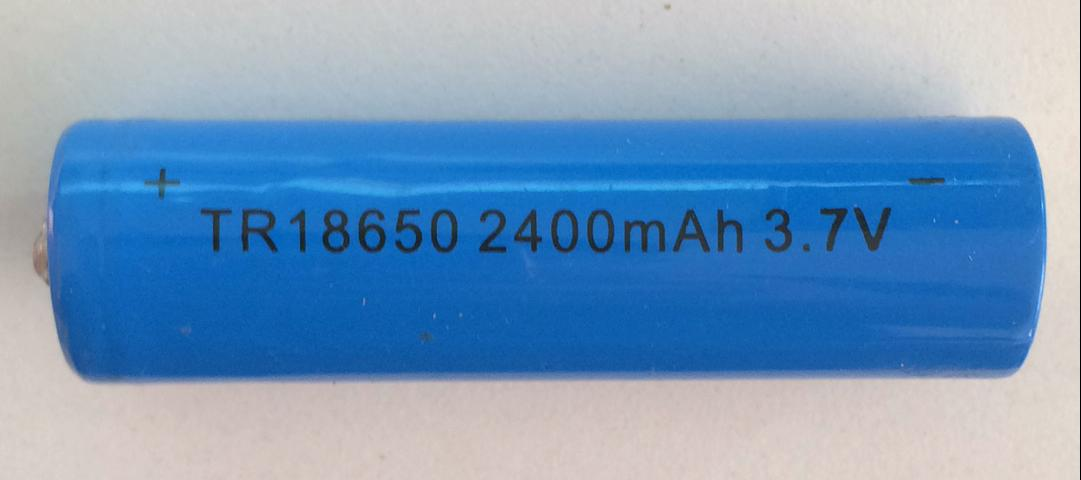
\includegraphics[width=0.9\textwidth]{./Figures/bateria.jpeg}			
	\caption{Batería TR18650 utilizada en el equipo}
	\label{fig:bateria}
\end{figure}

Teniendo en cuenta la eficiencia del 90\% y el porcentaje de descarga máxima de 51.35\%, la autonomía aprovechable de la batería será aproximadamente de 1109mAh, según lo calculado en la fórmula \ref{eqn:autonomiaReal}.
Este valor está cerca del consumo teórico calculado. 
\begin{equation} \label{eqn:autonomiaReal}
\begin{split}
autonomiaReal = autonomiaReal*eficiencia*porcentajeDescarga = \\ 2400mAh * 90\% * 51.35\% = 1109 mAh
\end{split}
\end{equation}

Se realizó un ensayo de la autonomía real del equipo siguiendo la secuencia normal de ensayo 
